
\documentclass[10pt,usenames,dvipsnames]{beamer}

\usetheme[progressbar=frametitle]{metropolis}
\usepackage{appendixnumberbeamer}

\usepackage{ulem}
\usepackage{pgfpages}
%\setbeamertemplate{note page}[plain]
%\setbeameroption{show notes on second screen=right}

\usepackage{booktabs}
\usepackage[scale=2]{ccicons}
\usepackage{todonotes}
\usepackage{amsmath} %added
\usepackage{bm}%added
%\usepackage{algorithm,algpseudocode}
\usepackage[]{algorithm2e}

\usepackage{subfig}
\usepackage{pgfplots}
\usepgfplotslibrary{dateplot}

\usepackage{tikz}%added
\usetikzlibrary{shapes,arrows}

\usepackage{booktabs}
\newcommand{\ra}[1]{\renewcommand{\arraystretch}{#1}}%added

\usepackage[export]{adjustbox}

\usepackage{wasysym}
%\usepackage{subcaption}


\usepackage{xspace}
\newcommand{\themename}{\textbf{\textsc{metropolis}}\xspace}

\title{Practical Session 2:}
\subtitle{Learning from Simulation for Malaria Control}
% \date{\today}
\date{}
\author{Presented by Sekou L. Remy}
\institute{Policy Making with AI, IBM Research$|$Africa}
% \titlegraphic{\hfill\includegraphics[height=1.5cm]{logo.pdf}}
% Let's get started
\begin{document}

\begin{frame}
  \titlepage
\end{frame}

\begin{frame}{Outline}

\setbeamertemplate{section in toc}[sections numbered]
\tableofcontents[hideallsubsections]
  % You might wish to add the option [pausesections]
\end{frame}

% Section and subsections will appear in the presentation overview
% and table of contents.

\section{Malaria Policy Decisions}

\subsection{Problem}


\begin{frame}{Malaria Prevention and Control}
\begin{itemize}

\item Disproportionate share of the global malaria burden in Sub Saharan Africa (SSA): 90\% malaria cases and 92\% deaths 

\item SSA countries rely heavily on external funding for malaria prevention and control \cite{Winskill2011}

\item  \$450M in R\&D spent each year, slower growth after 2018 \cite{moran2007malaria}

\item With tools that maximize the cost-effectiveness of malaria interventions, there is the potential to drive transformation

\end{itemize}

%\begin{figure}[h]
% 
%\begin{subfigure}{0.5\textwidth}
%
\includegraphics[width=0.9\linewidth, height=5cm]{images/AMF.png} 
%\caption{Caption1}
%\label{fig:subim1}
%\end{subfigure}
%\begin{subfigure}{0.5\textwidth}
%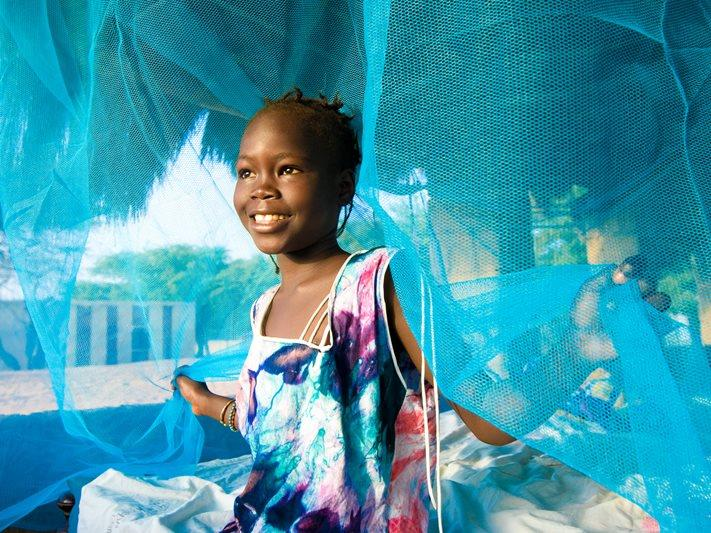
\includegraphics[width=0.9\linewidth, height=5cm]{images/Bednet.jpeg}
%\caption{Caption 2}
%\label{fig:subim2}
%\end{subfigure}
% 
%\caption{Caption for this figure with two images}
%\label{fig:image2}
%\end{figure}

\centering
        \begin{tabular}{ccc}
        
        
\includegraphics[width=3cm]{images/AMF.png}
        &
         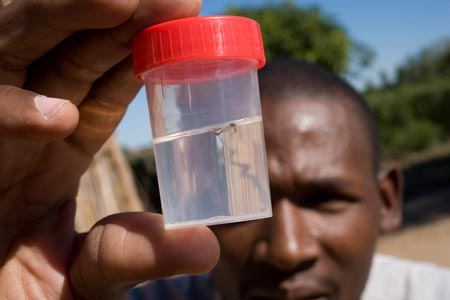
\includegraphics[width=4cm]{images/Research.jpg}
         &
         
\includegraphics[width=2.5cm]{images/BillM.jpg}
        
      \end{tabular}
      
      \url{http://www.who.int/mediacentre/factsheets/fs094/en/}



%
\includegraphics[width=0.45\textwidth]{images/AMF.png}
%
%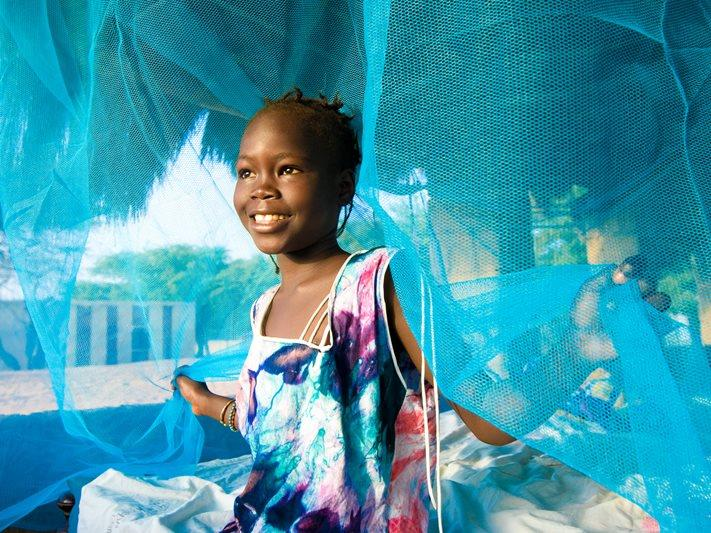
\includegraphics[width=0.45\textwidth, right]{images/Bednet.jpeg}
%
%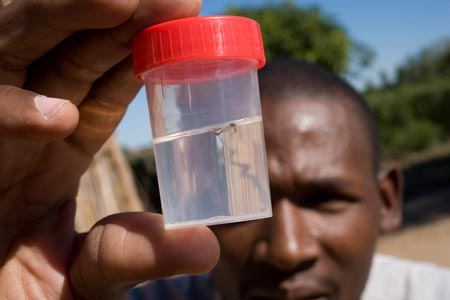
\includegraphics[width=0.45\textwidth]{images/Research.jpg}
%
%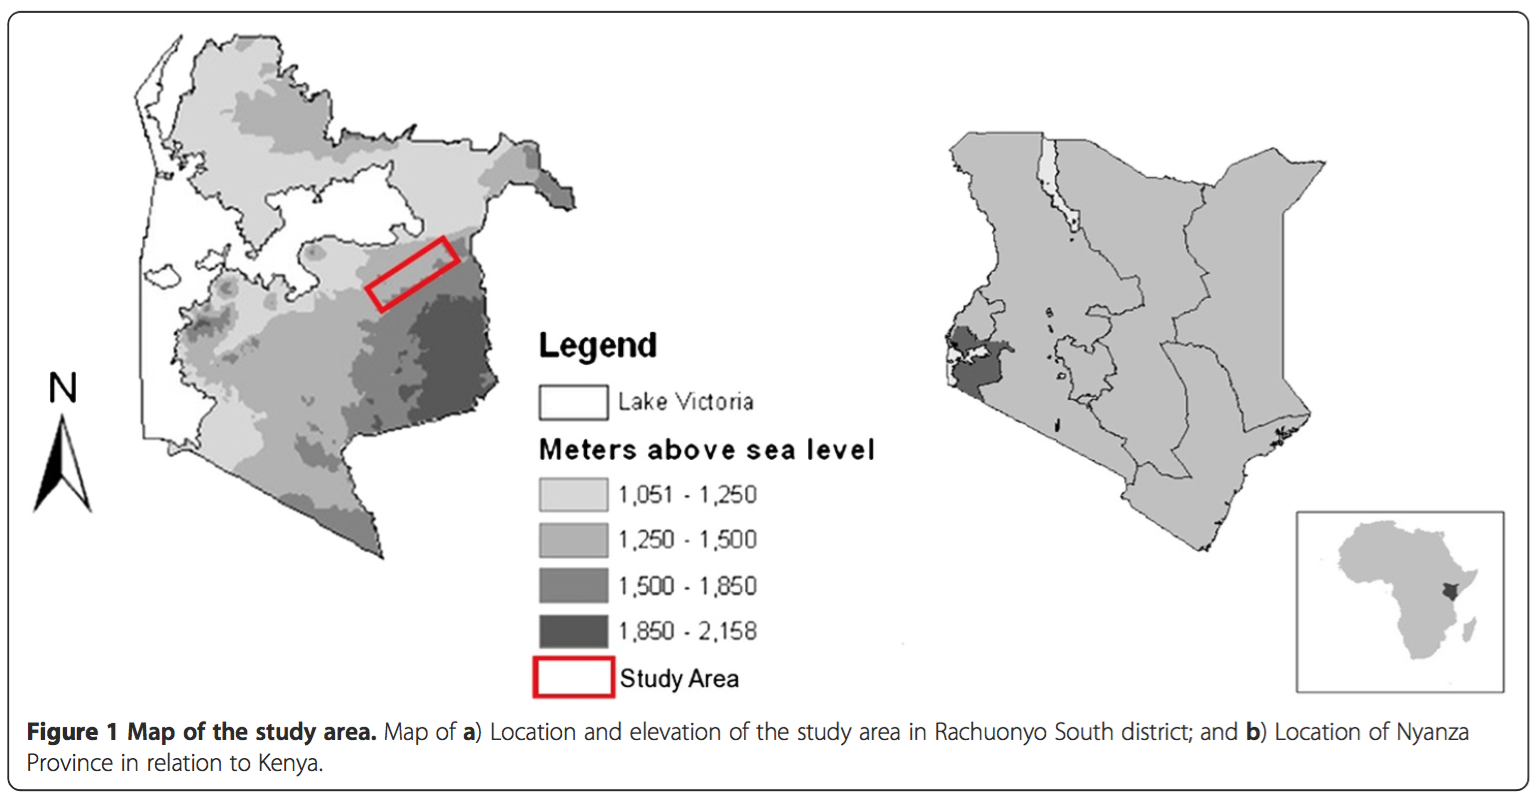
\includegraphics[width=0.45\textwidth]{images/WesternKenya.png}



\end{frame}

\subsubsection{Application}

% You can reveal the parts of a slide one at a time
% with the \pause command:
\begin{frame}{Decision Makers and Interventions}

\begin{itemize}
\item Currently different decision makers (e.g., NGOs, Governments and Charities), independently explore interventions
\item Policies include mixed interventions eg. distribution of long-lasting insecticide-treated nets (ITNs), indoor residual spraying (IRS), vector larviciding, and vaccinations
\item The space of all policies for malaria interventions is growing, making informed decisions harder 
\item \textit{Are humans the best single decision-makers?}
\end{itemize}

\centering
        \begin{tabular}{ccc}
        
        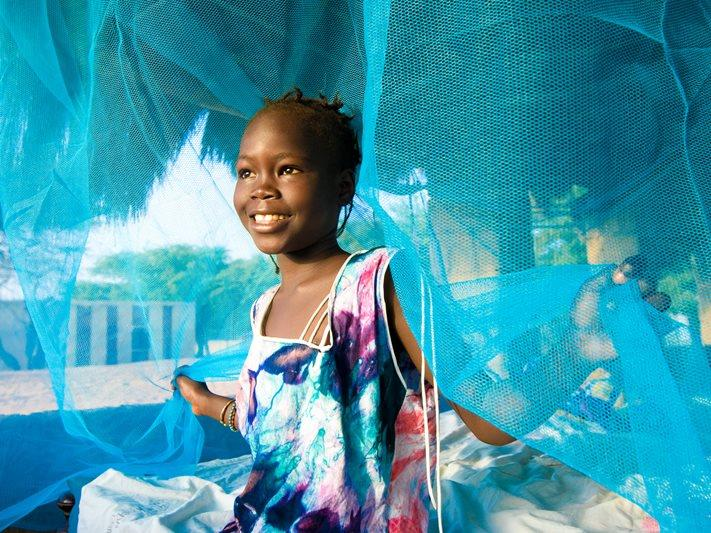
\includegraphics[width=3cm]{images/Bednet.jpeg}
        &
         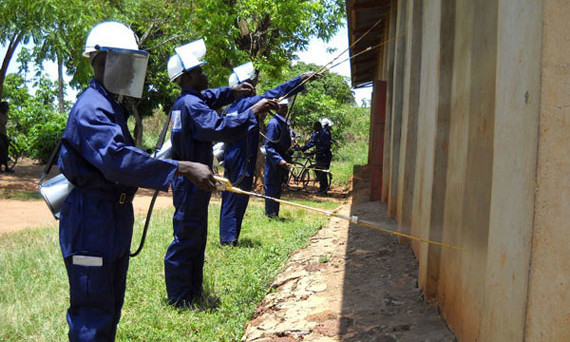
\includegraphics[width=4cm]{images/IRS.jpg}
         &
         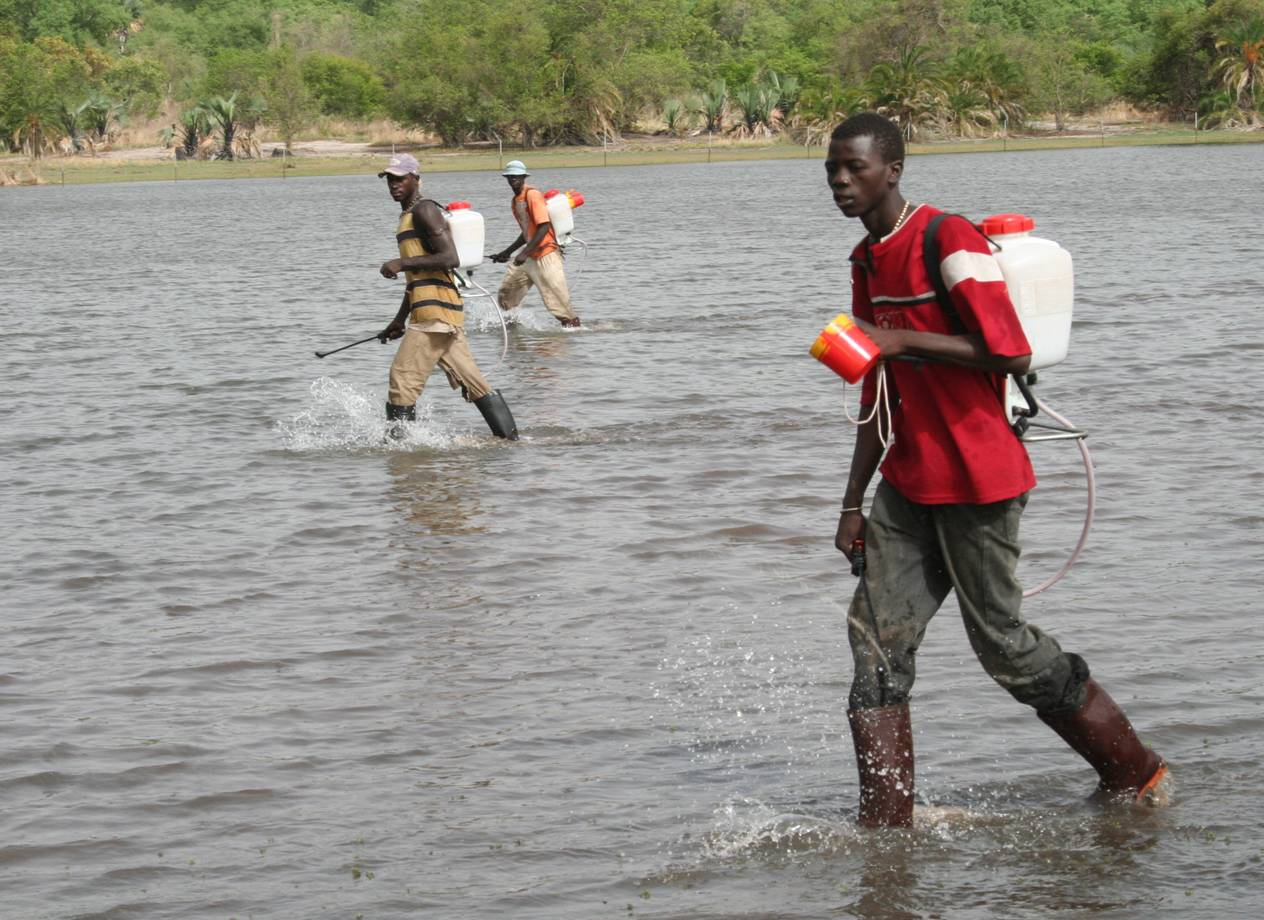
\includegraphics[width=3cm]{images/larv.jpeg}
        
      \end{tabular}

\end{frame}
%
%\subsubsection{Related Work}
%
%% You can reveal the parts of a slide one at a time
%% with the \pause command:
%\begin{frame}{Existing Research for Decision-Making (Geospatial)}
%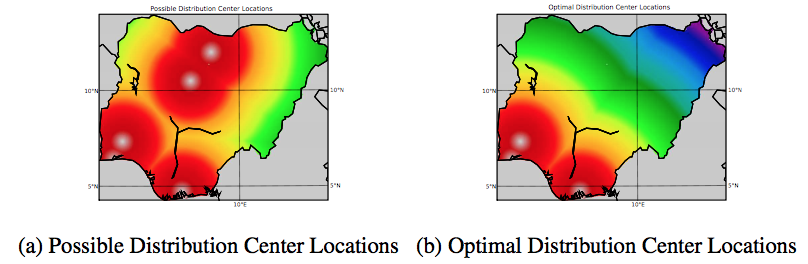
\includegraphics[width=1\textwidth]{images/nigeria.png}
%
%
%\centering
%        \begin{tabular}{cc}
%        
%        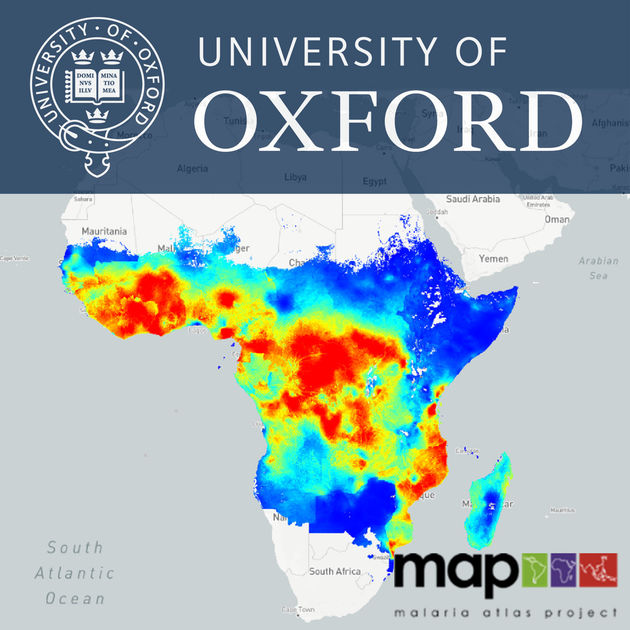
\includegraphics[width=4cm]{images/OxfordMaps.jpg}
%        &
%         
\includegraphics[width=5cm]{images/disarm.jpg}
%        
%      \end{tabular}
%
%\begin{itemize}
%\item \cite{Piette2016}, \cite{Dimitrov2009}
%
%\end{itemize}
%
%
%\end{frame}

\subsubsection{OpenMalaria}

% You can reveal the parts of a slide one at a time
% with the \pause command:
\begin{frame}{Simulation and Modeling Overview}


\begin{itemize}
\item Separate from modeling geospatial interactions, this work uses open-source models of the interactions between humans, mosquitoes (vectors) and the malaria parasite
\item OpenMalaria \cite{SMITH2008a}, provides stochastic transmission models of malaria 
\item Used by researchers to evaluate the impact of various malaria control interventions on simulated Human populations, for single environments

\end{itemize}

\centering
 \begin{tabular}{cc}
        
        
\includegraphics[width=4cm]{images/GH.png}
        &
         
\includegraphics[width=5cm]{images/swiss.jpg}
        
      \end{tabular}

\end{frame}

% You can reveal the parts of a slide one at a time
% with the \pause command:

\begin{frame}{Example Stochastic Simulation in Human Populations}
\hspace{1cm}
\centering{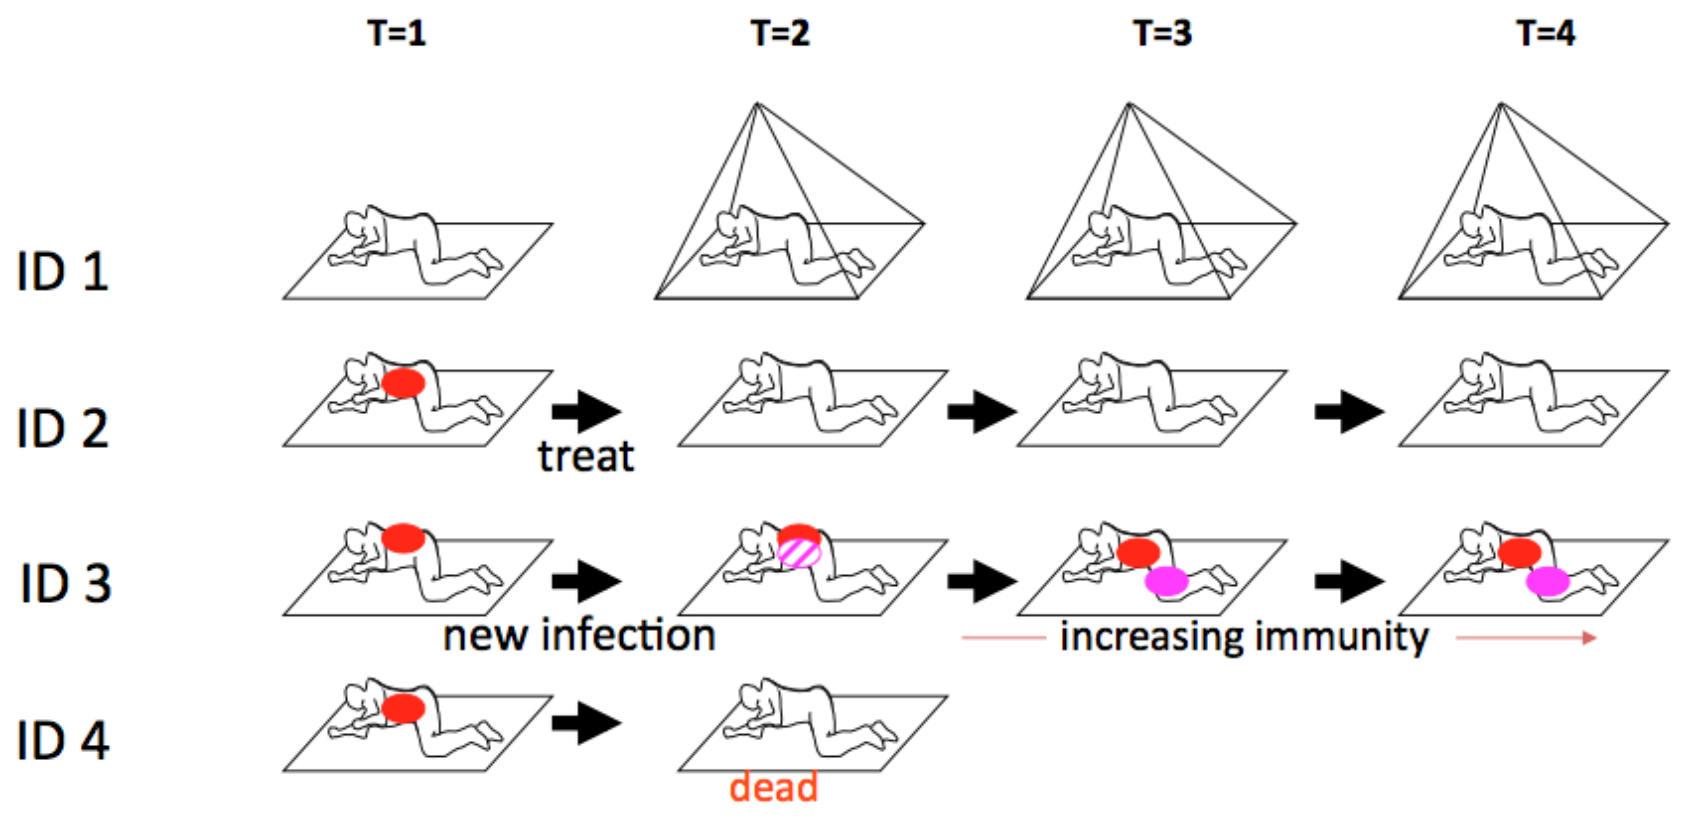
\includegraphics[width=1\textwidth]{images/Humans.png}}
 

\cite{Stuckey2012}


\end{frame}

\begin{frame}{Example Deterministic Models for Vector Control}
\hspace{1cm}
\centering
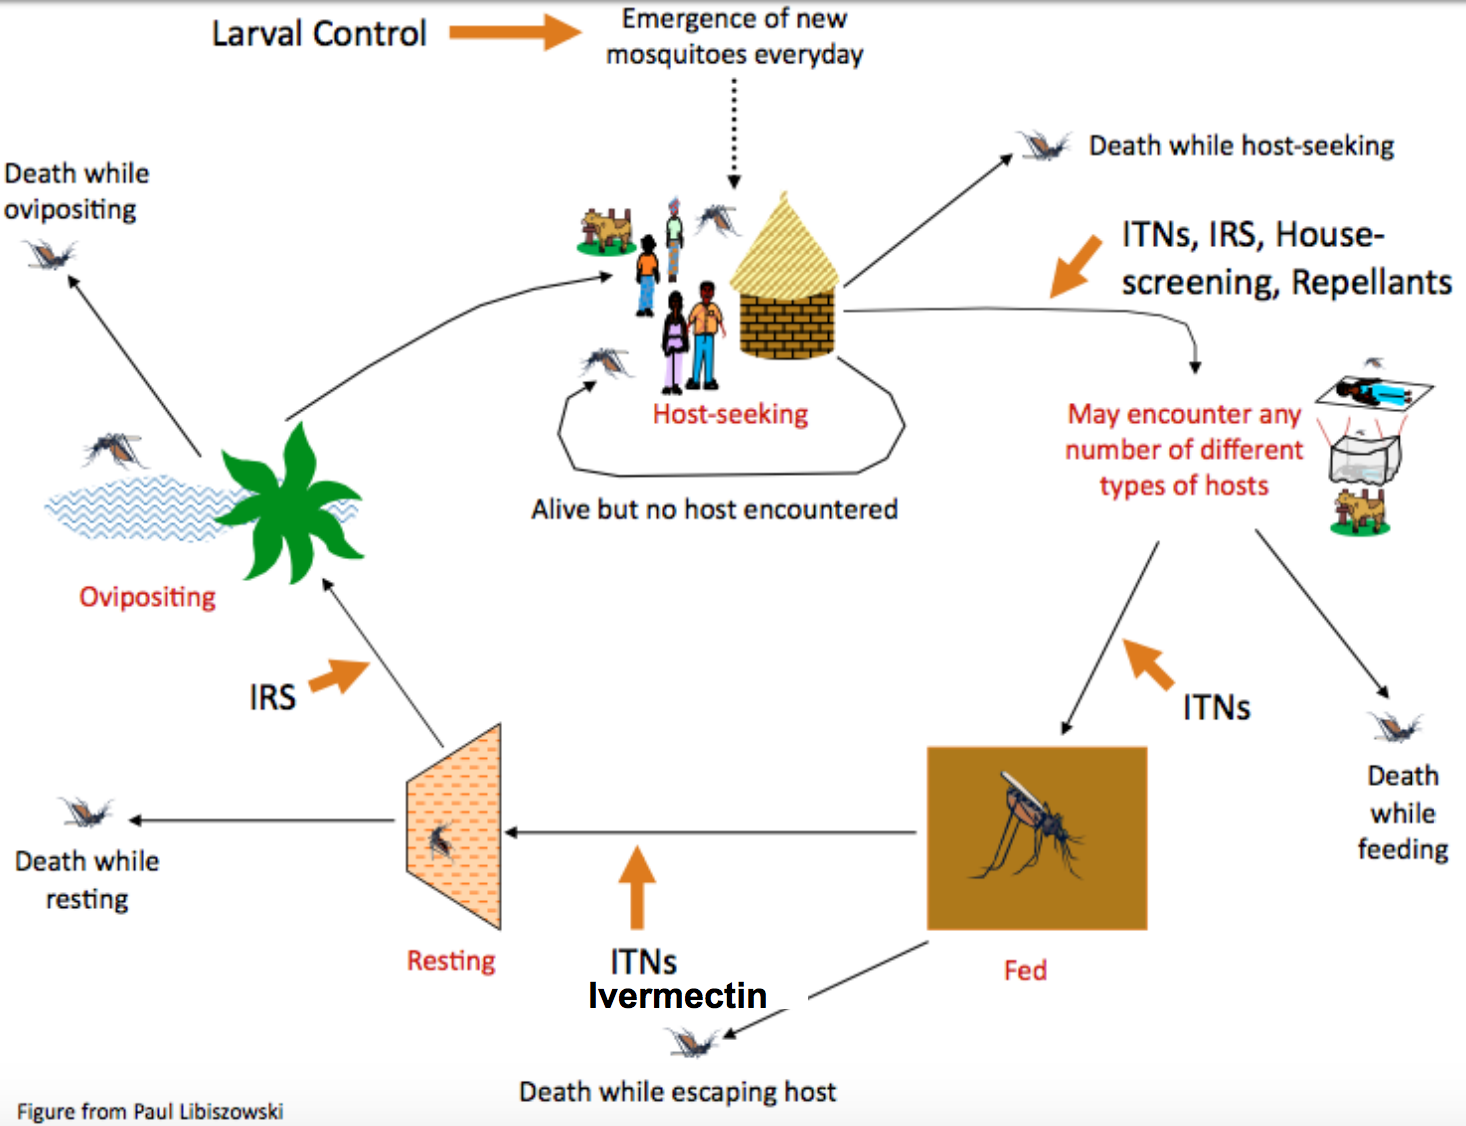
\includegraphics[width=.9\textwidth]{images/MosquitoLifeCycle.png}


\end{frame}


\begin{frame}{Example Evaluation of 5 policies}
\hspace{1cm}

\centering{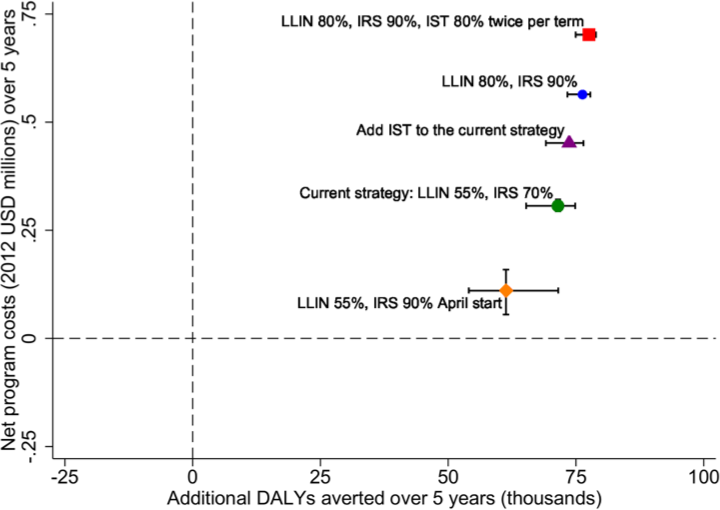
\includegraphics[width=.8\textwidth]{images/HealthPolicy.png}}

\cite{Stuckey2014}

\end{frame}

\subsection{Novel Solution?}

%\subsection{Complete Problem Formulation}

% You can reveal the parts of a slide one at a time
% with the \pause command:
\begin{frame}{Novel Exploration Techniques (NETs) for Malaria Policy Interventions}

\begin{itemize}
\item Proposing a novel formulation for the exploration of malaria intervention actions, for Rachuonyo South District - Kenya 
\item You implement algorithms which learn from this problem formulation in the Reinforcement Learning paradigm
\end{itemize}
\centering
         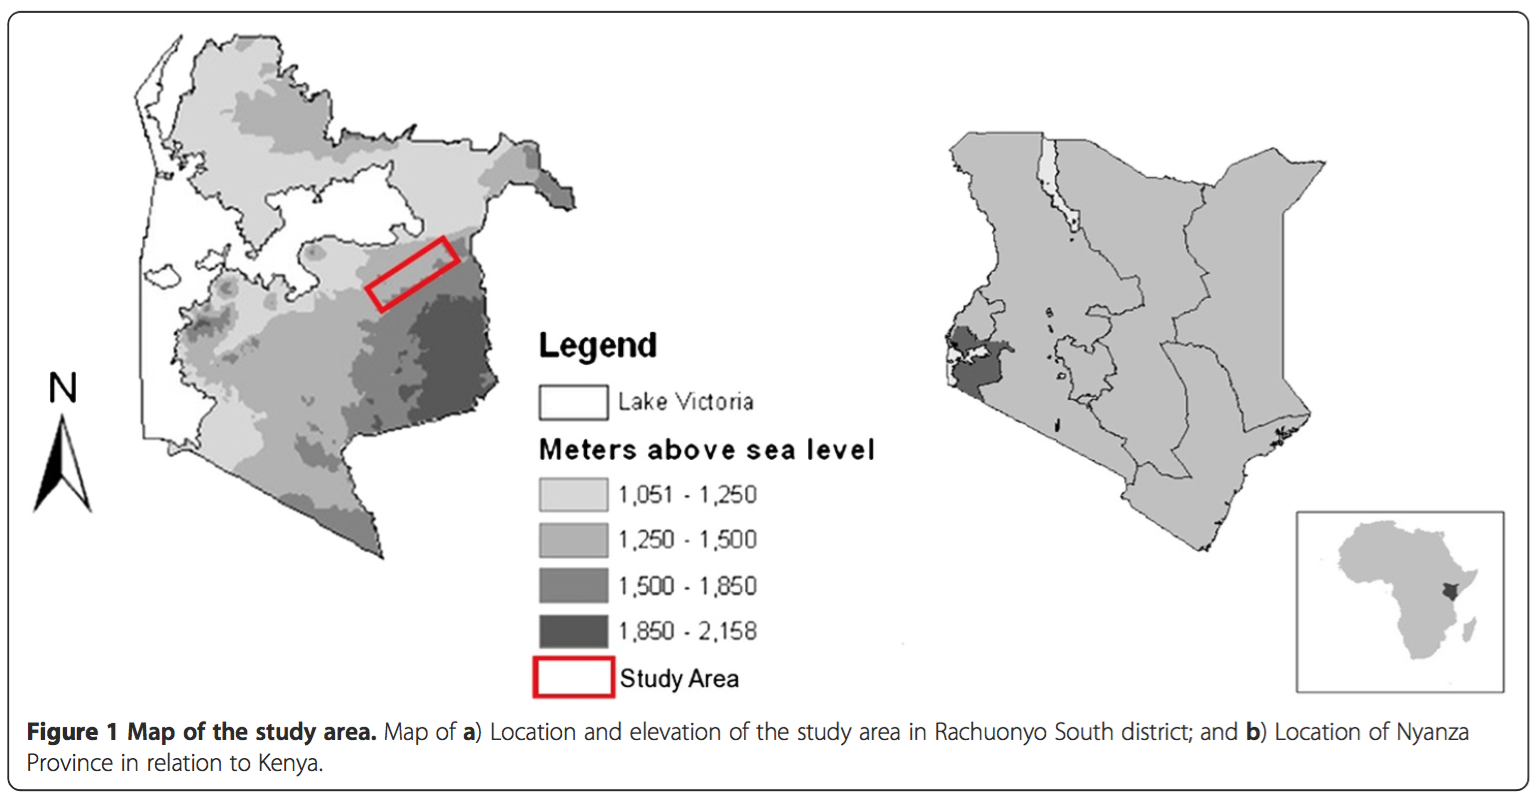
\includegraphics[width=7cm]{images/WesternKenya.png} 
\end{frame}



\section{Problem Formulation}

\subsection{Stochastic Multi-Armed Bandit}
\begin{frame}{Stochastic Multi-Armed Bandit (MAB)}

\begin{itemize}
\item We engineered OpenMalaria to create a simulation environment.
\item Site specific parameterisation ($\theta$) already performed by humans \cite{Stuckey2012}
\item Historically MAB algorithms have been used to develop models for the design of clinical trials, where actions should balance exploitation (positive patient outcomes) and exploration (towards a clinical `breakthrough')
\item  Determine high performing policies for a simulated population in Rachuonyo South for the next 5 years
\end{itemize}

\begin{figure}[!t]
\centering
\tikzstyle{OMenvironment} = [rectangle, draw, fill=blue!20, 
    text width=6em, text centered, rounded corners, minimum height=4em]
\tikzstyle{line} = [draw, -latex']
\tikzstyle{Agent Model} = [draw, ellipse,fill=red!20, node distance=3cm,
    minimum height=2em]
    
\begin{tikzpicture}[node distance = 4cm, auto]
    % Place nodes

    \node [Agent Model] (Agent) {Agent Model};
    \node [OMenvironment, right of=Agent] (env) {OpenMalaria Simulation Environment};

    % Draw edges

    \path[line] (env) |-([shift={(3mm,-3mm)}]env.south west)-- node [shift = {(3mm,0mm)}]{$R_{\theta}(\bm{a}_i)$} ([shift={(3mm,-6mm)}]Agent.south)-|(Agent);
    
      \path[line] (Agent) |-([shift={(-3mm,7.25mm)}]Agent.north east)-- node [shift = {(-3mm,0mm)}]{$\bm{a}_i$}([shift={(-3mm,3mm)}]env.north)-|(env);


\end{tikzpicture}
%\caption{Policies $\bm{a}_i$ are chosen by the Agent Model which receives Rewards $R(\bm{a}_i)$}
\label{fig_flow}
\end{figure}

\end{frame}

%\subsubsection{State}
\begin{frame}{State}

\begin{itemize}
\item MAB is a subset of the full Reinforcement Learning problem
\item State is defined by the simulation's initial parameters $\theta$ and the policy of interventions $\bm{a}$ simulated (single `Bandit' arm)
\item No notion of state transition between OpenMalaria simulations (arms)
\item Solving for the problem of making a \textbf{one-shot} policy decision for the next 5 years in Rachuonyo South

\end{itemize}

\begin{figure}[!t]
\centering
\tikzstyle{OMenvironment} = [rectangle, draw, fill=blue!20, 
    text width=6em, text centered, rounded corners, minimum height=4em]
\tikzstyle{line} = [draw, -latex']
\tikzstyle{Agent Model} = [draw, ellipse,fill=red!20, node distance=3cm,
    minimum height=2em]
    
\begin{tikzpicture}[node distance = 4cm, auto]
    % Place nodes

    \node [Agent Model] (Agent) {Agent Model};
    \node [OMenvironment, right of=Agent] (env) {OpenMalaria Simulation Environment};

    % Draw edges

    \path[line] (env) |-([shift={(3mm,-3mm)}]env.south west)-- node [shift = {(3mm,0mm)}]{$R_{\theta}(\bm{a}_i)$} ([shift={(3mm,-6mm)}]Agent.south)-|(Agent);
    
      \path[line] (Agent) |-([shift={(-3mm,7.25mm)}]Agent.north east)-- node [shift = {(-3mm,0mm)}]{$\bm{a}_i$}([shift={(-3mm,3mm)}]env.north)-|(env);


\end{tikzpicture}
%\caption{Policies $\bm{a}_i$ are chosen by the Agent Model which receives Rewards $R(\bm{a}_i)$}
\label{fig_flow}
\end{figure}



\end{frame}

%\subsubsection{Action}
\begin{frame}{Action}

\begin{itemize}
\item Mass-distribution of insecticide-treated nets ($a_{ITN} \in (0,1]$)
\item Seasonal Indoor Residual Spraying with pyrethroids ($a_{IRS}\in (0,1]$)
\item Prompt and effective treatment of malaria  \cite{Stuckey2014}
\end{itemize}
\begin{equation}
\bm{a}_i \in A = \{a_{ITN}, a_{IRS}\}
\end{equation}

\begin{figure}[!t]
\centering
\tikzstyle{OMenvironment} = [rectangle, draw, fill=blue!20, 
    text width=6em, text centered, rounded corners, minimum height=4em]
\tikzstyle{line} = [draw, -latex']
\tikzstyle{Agent Model} = [draw, ellipse,fill=red!20, node distance=3cm,
    minimum height=2em]
    
\begin{tikzpicture}[node distance = 4cm, auto]
    % Place nodes

    \node [Agent Model] (Agent) {Agent Model};
    \node [OMenvironment, right of=Agent] (env) {OpenMalaria Simulation Environment};

    % Draw edges

    \path[line] (env) |-([shift={(3mm,-3mm)}]env.south west)-- node [shift = {(3mm,0mm)}]{$R_{\theta}(\bm{a}_i)$} ([shift={(3mm,-6mm)}]Agent.south)-|(Agent);
    
      \path[line] (Agent) |-([shift={(-3mm,7.25mm)}]Agent.north east)-- node [shift = {(-3mm,0mm)}]{$\bm{a}_i$}([shift={(-3mm,3mm)}]env.north)-|(env);


\end{tikzpicture}
%\caption{Policies $\bm{a}_i$ are chosen by the Agent Model which receives Rewards $R(\bm{a}_i)$}
\label{fig_flow}
\end{figure}

\end{frame}

%\begin{frame}{Actions - Challenges}
%
%OpenMalaria provides a stochastic distribution of interventions across the simulated population. These decisions are \textit{not} made in a targeted manor:
%\begin{itemize}
%\item Time dependent
%\item Cohort dependent
% 
%\end{itemize}
%Policy space grows exponentially with number of interventions or intervention variables. Compute time growing linearly with number of simulated individuals.
%
%\begin{figure}[!t]
%\centering
%\tikzstyle{OMenvironment} = [rectangle, draw, fill=blue!20, 
%    text width=6em, text centered, rounded corners, minimum height=4em]
%\tikzstyle{line} = [draw, -latex']
%\tikzstyle{Agent Model} = [draw, ellipse,fill=red!20, node distance=3cm,
%    minimum height=2em]
%    
%\begin{tikzpicture}[node distance = 4cm, auto]
%    % Place nodes
%
%    \node [Agent Model] (Agent) {Agent Model};
%    \node [OMenvironment, right of=Agent] (env) {OpenMalaria Simulation Environment};
%
%    % Draw edges
%
%    \path[line] (env) |-([shift={(3mm,-3mm)}]env.south west)-- node [shift = {(3mm,0mm)}]{$R_{\theta}(\bm{a}_i)$} ([shift={(3mm,-6mm)}]Agent.south)-|(Agent);
%    
%      \path[line] (Agent) |-([shift={(-3mm,7.25mm)}]Agent.north east)-- node [shift = {(-3mm,0mm)}]{$\bm{a}_i$}([shift={(-3mm,3mm)}]env.north)-|(env);
%
%
%\end{tikzpicture}
%%\caption{Policies $\bm{a}_i$ are chosen by the Agent Model which receives Rewards $R(\bm{a}_i)$}
%\label{fig_flow}
%\end{figure}
%
%\end{frame}


% Placing a * after \section means it will not show in the
% outline or table of contents.

\subsection{Reward}

\begin{frame}{Reward}

\begin{itemize}
\item $R_\theta(\bm{a}_i)$ is stochastic through the parameterisation of the simulation $\theta$
\item $\theta$ defines a randomised distribution of parameters for the simulation.
\item The magnitude of the reward has been determined through an economic cost-effectiveness analysis of the simulation output
\end{itemize}

% \textit(note) include something on reward clipping for stability.

\begin{figure}[!t]
\centering
\tikzstyle{OMenvironment} = [rectangle, draw, fill=blue!20, 
    text width=6em, text centered, rounded corners, minimum height=4em]
\tikzstyle{line} = [draw, -latex']
\tikzstyle{Agent Model} = [draw, ellipse,fill=red!20, node distance=3cm,
    minimum height=2em]
    
\begin{tikzpicture}[node distance = 4cm, auto]
    % Place nodes

    \node [Agent Model] (Agent) {Agent Model};
    \node [OMenvironment, right of=Agent] (env) {OpenMalaria Simulation Environment};

    % Draw edges

    \path[line] (env) |-([shift={(3mm,-3mm)}]env.south west)-- node [shift = {(3mm,0mm)}]{$R_{\theta}(\bm{a}_i)$} ([shift={(3mm,-6mm)}]Agent.south)-|(Agent);
    
      \path[line] (Agent) |-([shift={(-3mm,7.25mm)}]Agent.north east)-- node [shift = {(-3mm,0mm)}]{$\bm{a}_i$}([shift={(-3mm,3mm)}]env.north)-|(env);


\end{tikzpicture}
%\caption{Policies $\bm{a}_i$ are chosen by the Agent Model which receives Rewards $R(\bm{a}_i)$}
\label{fig_flow}
\end{figure}

\end{frame}

%\subsubsection{DALYs}


%\subsubsection{Cost Effectiveness}

\begin{frame}{Cost Effectiveness of Interventions}

\begin{itemize}
\item The proposed algorithm will receive rewards based on the \textit{cost effectiveness} of a policy, this metric is one of many used by researchers evaluating the impact of policy decisions
\item  Cost effectiveness will be evaluated as the cost per DALY averted $C_{DA}$
\end{itemize}

\begin{equation}
C_{DA} =\dfrac{C_{\mbox{int}} + HSC_{\mbox{int}}-HSC_{\mbox{no~int}}}{DALYs_{int}-DALYs_{no~int}} 
\end{equation}


\end{frame}


\subsection{Example Scenario: Rachuonyo South }

\begin{frame}{Example Scenario: Rachuonyo South}

\begin{itemize}
\item Current Implementation: 55\% ITNs ($a_{ITN} = 0.55$) and 70\% IRS ($a_{IRS} = 0.7$) 
	\begin{itemize}
	\item Researchers assess this as most cost-effective policy
	\end{itemize}
\item[ ]
\item \textit{If we train an algorithm directly on the simulation environment what can we learn about Rachuonyo South?}
\end{itemize}
\centering
         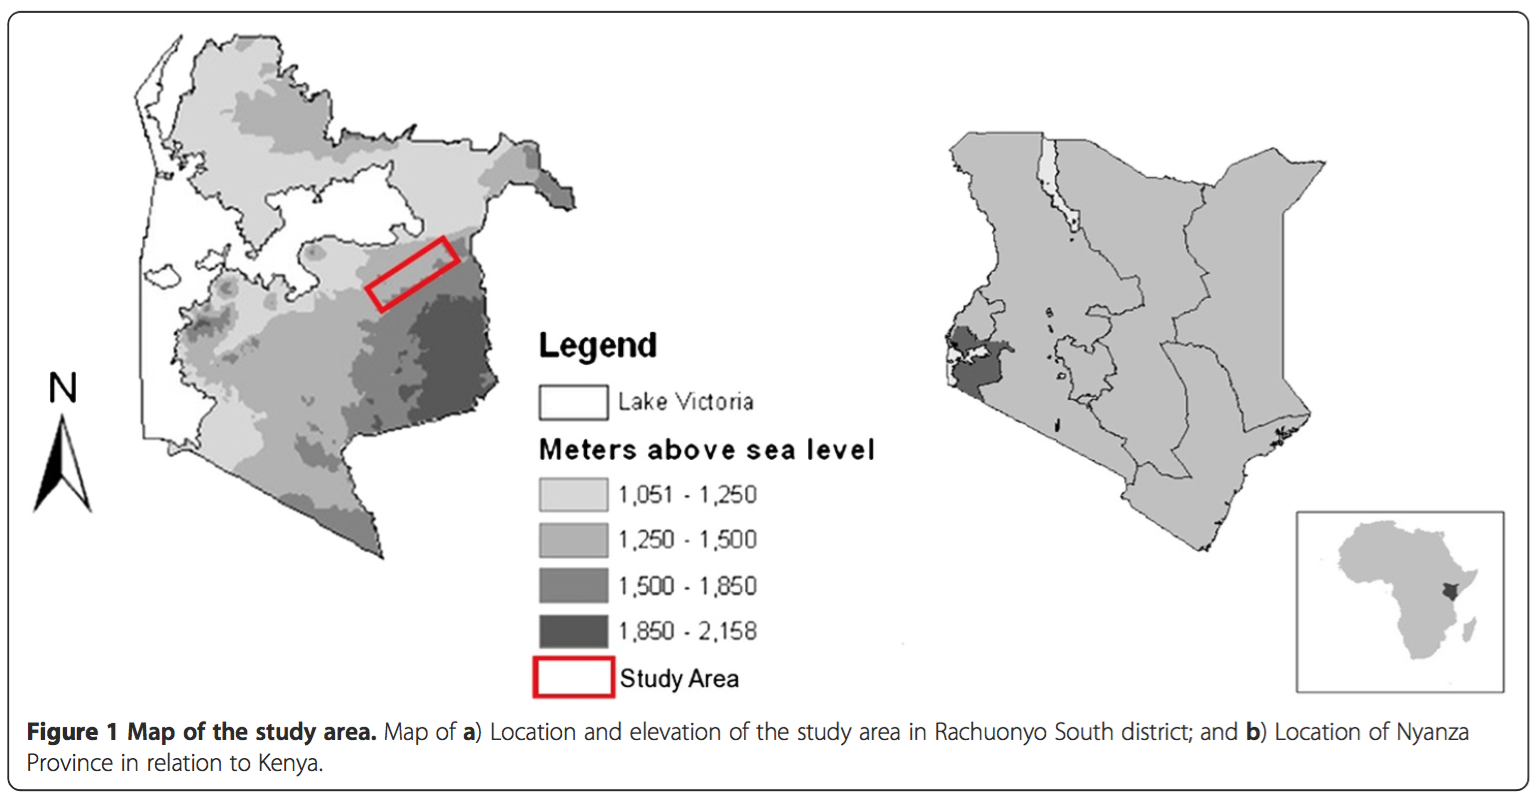
\includegraphics[width=7cm]{images/WesternKenya.png} 
         
\textit{note:} using a simulated population size 100,000
\end{frame}


%\begin{frame}{Example Policy Exploration Rachuonyo South}{Gaussian Processes for Sample-Efficiency and Inference}
%\centering
%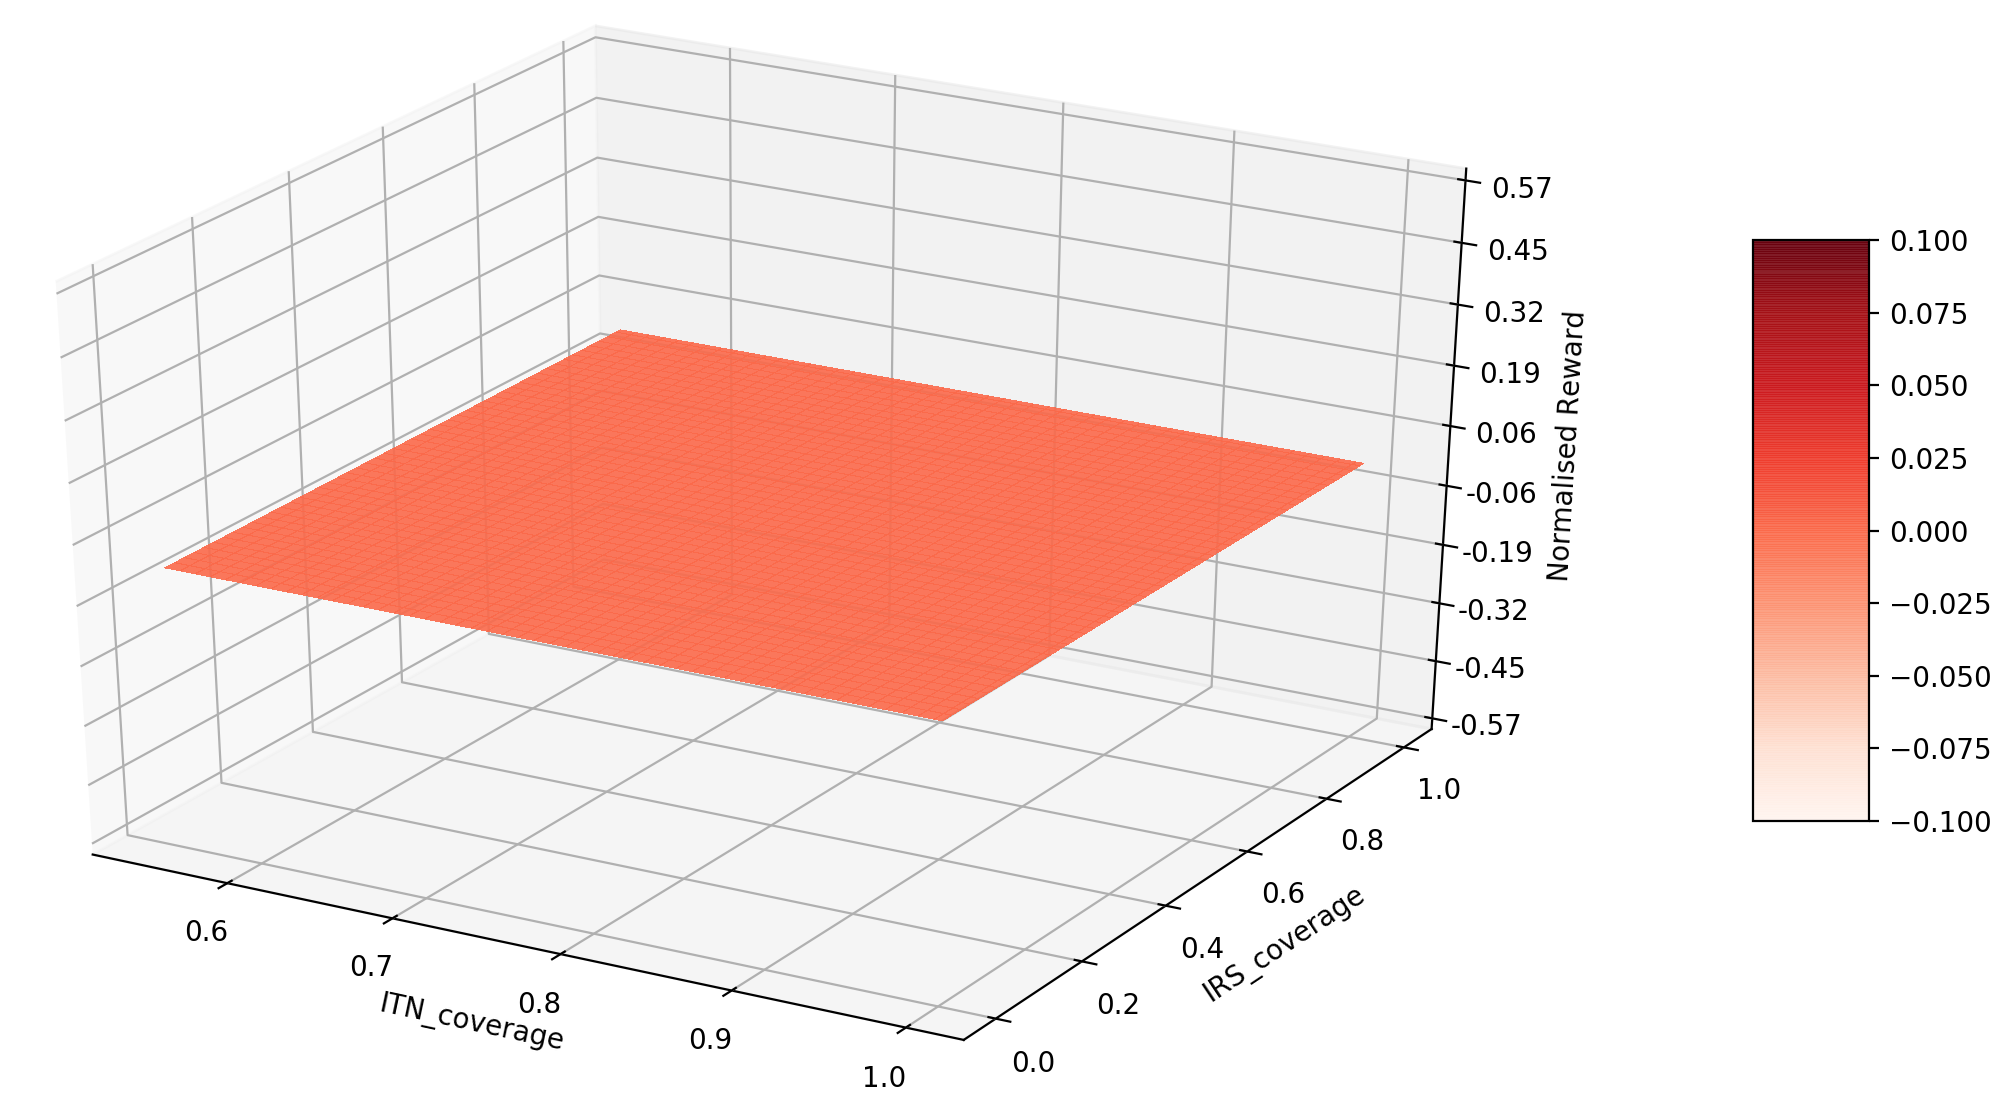
\includegraphics[width=1\textwidth]{images/Flatr.png}
%\end{frame}
\begin{frame}{Example Policy Exploration Rachuonyo South}{Gaussian Processes for Sample-Efficiency and Inference - First Random Sample}
\centering
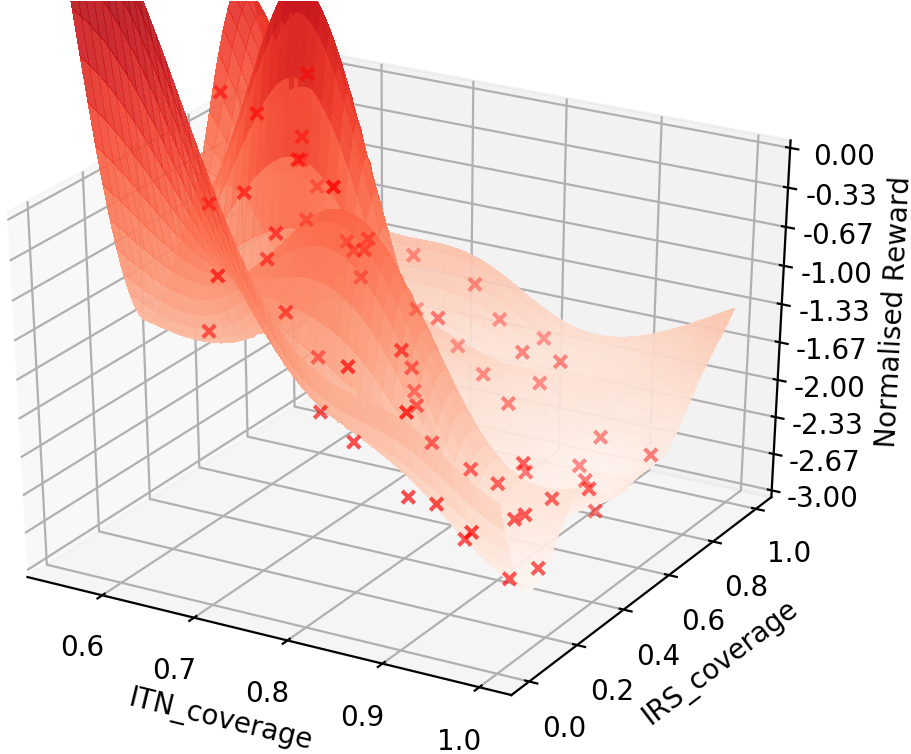
\includegraphics[width=1\textheight]{images/Batch_1.png}
\end{frame}
\begin{frame}{Example Policy Exploration Rachuonyo South}{Gaussian Processes for Sample-Efficiency and Inference - Second Sample}
\centering
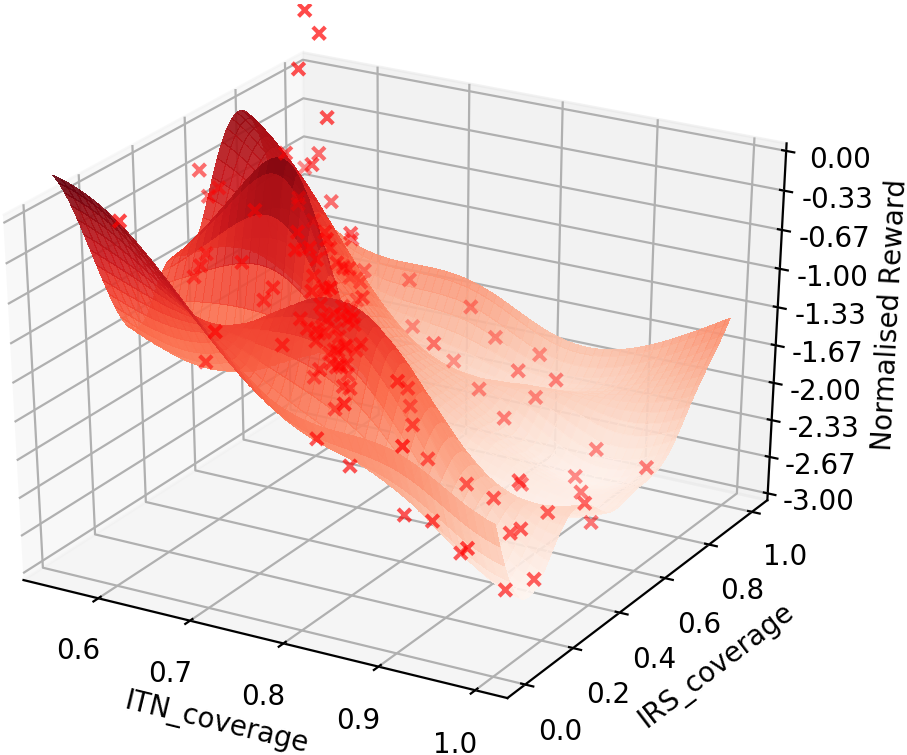
\includegraphics[width=1\textheight]{images/Batch_2.png}
\end{frame}
\begin{frame}{Example Policy Exploration Rachuonyo South}{Gaussian Processes for Sample-Efficiency and Inference}
\centering
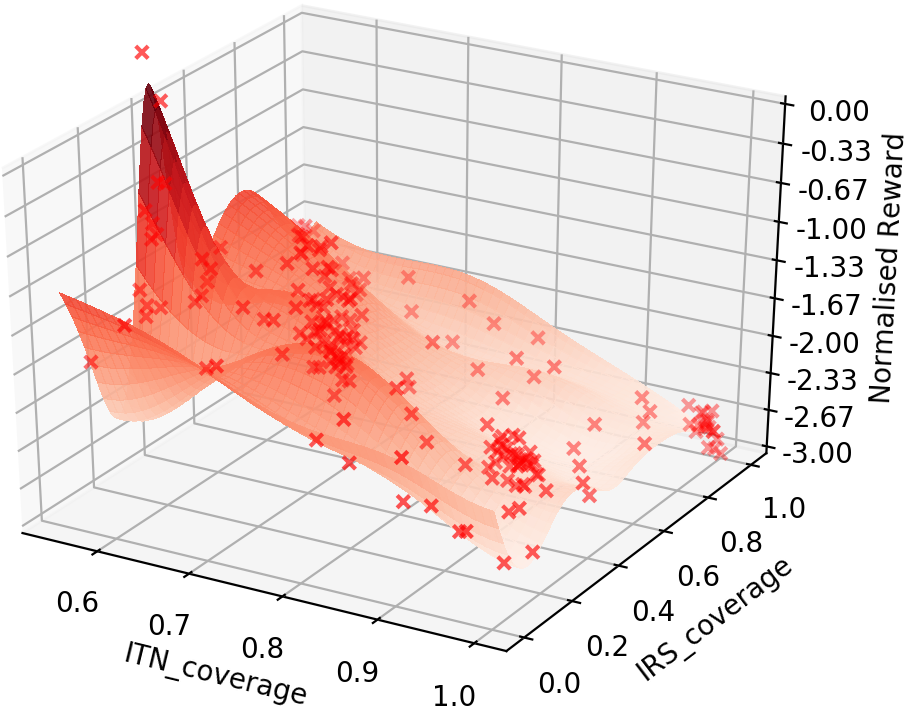
\includegraphics[width=1\textheight]{images/Batch_3.png}
\end{frame}
\begin{frame}{Example Policy Exploration Rachuonyo South}{Gaussian Processes for Sample-Efficiency and Inference}
\centering
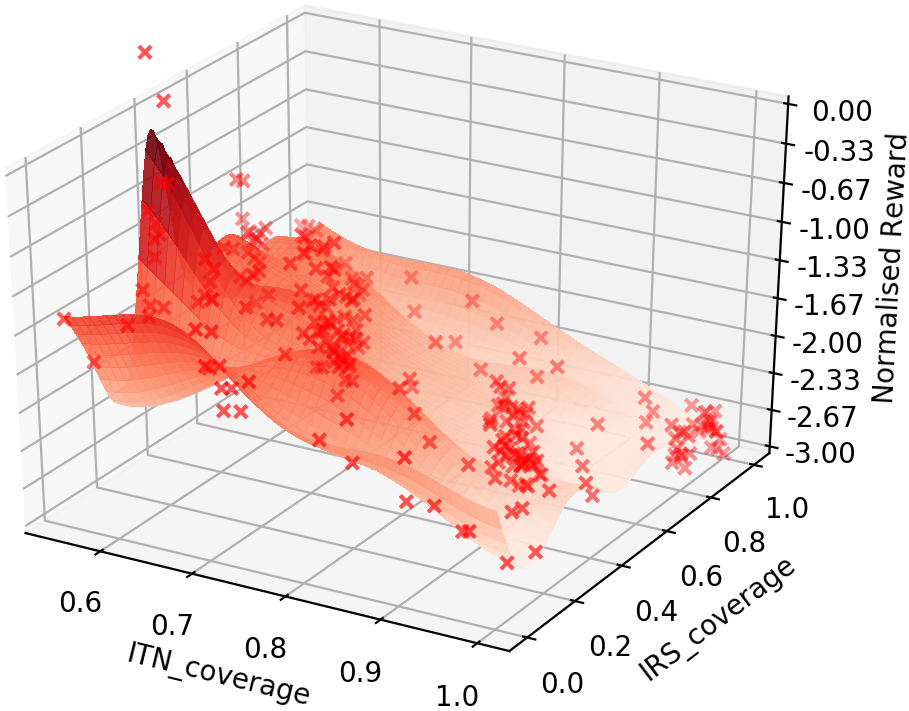
\includegraphics[width=1\textheight]{images/Batch_4.png}
\end{frame}
\begin{frame}{Example Policy Exploration Rachuonyo South}{Gaussian Processes for Sample-Efficiency and Inference}
\centering
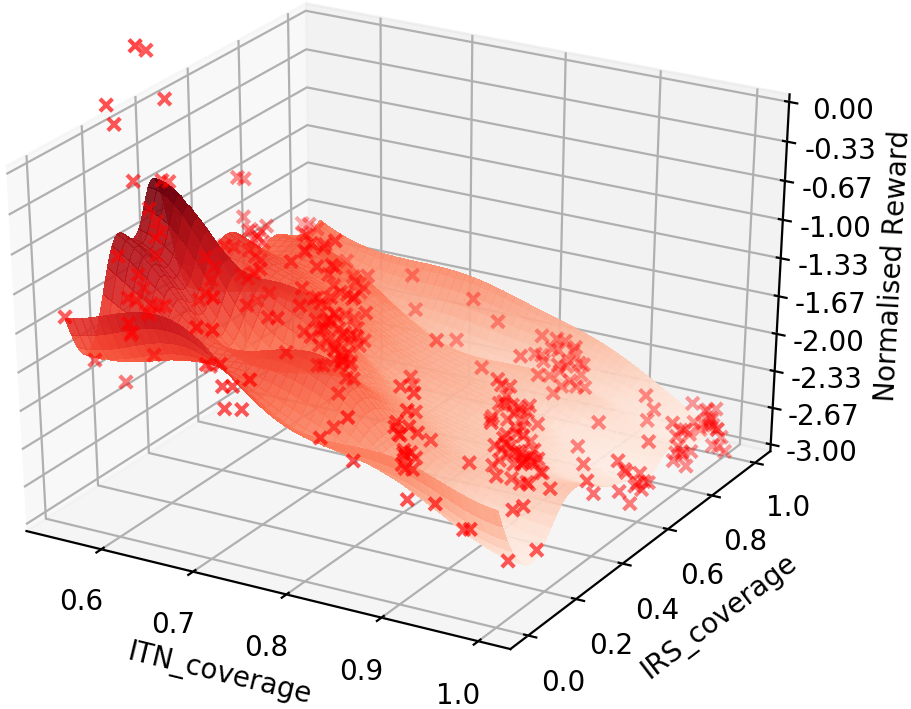
\includegraphics[width=1\textheight]{images/Batch_5.png}
\end{frame}
\begin{frame}{Example Policy Exploration Rachuonyo South}{Gaussian Processes for Sample-Efficiency and Inference}
\centering
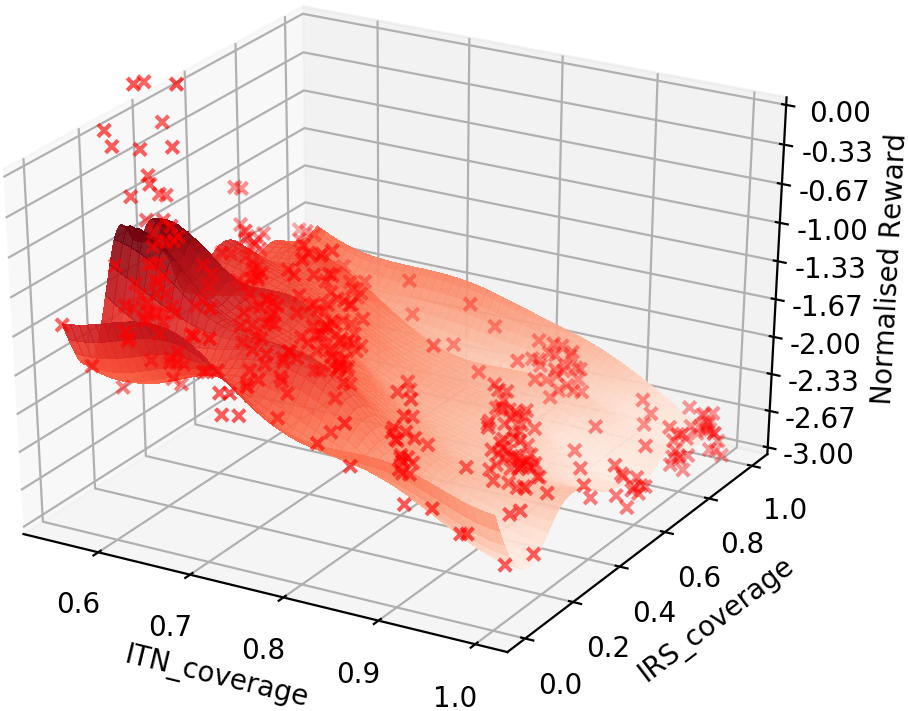
\includegraphics[width=1\textheight]{images/Batch_6.png}
\end{frame}
\begin{frame}{Example Policy Exploration Rachuonyo South}{Gaussian Processes for Sample-Efficiency and Inference}
\centering
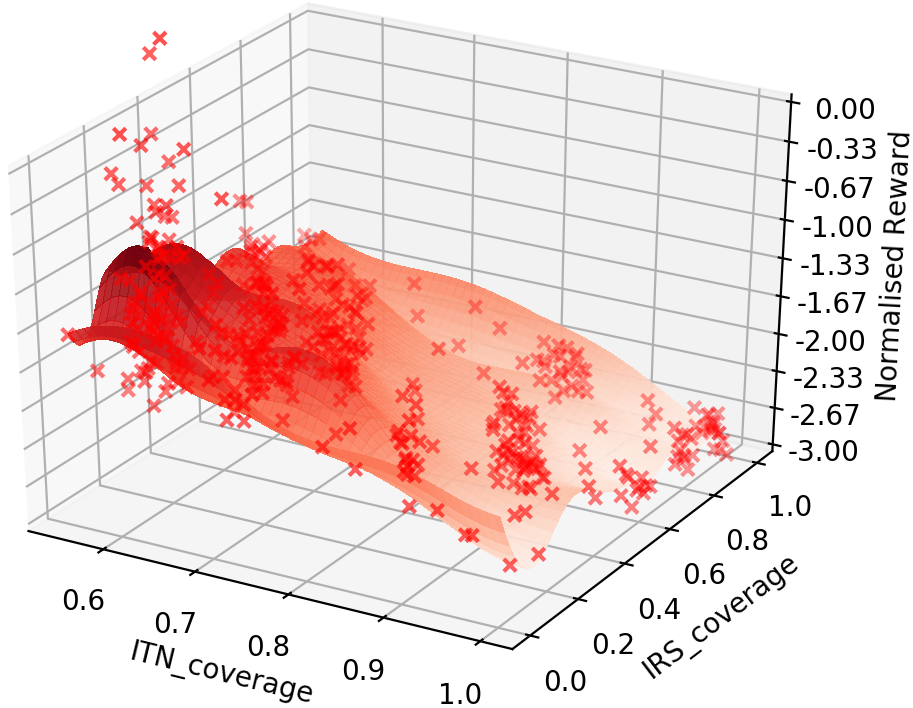
\includegraphics[width=1\textheight]{images/Batch_7.png}
\end{frame}



\subsection{System Implementation and Deployment}

\subsection{Agent Models}
\begin{frame}{Agent Models}
\begin{itemize}
\item Each algorithm performs sequential batch exploration, with the goal of optimisation of an unknown stochastic reward function $R$
\item At each batch we will choose $j=1,2,..,B$ policies $\bm{a}_i^j \in A$. Due to the computational expense of calculating $R(\bm{a}_i)$ and the size of the entire $A$, we wish to find solutions of maximal reward in as few iterations $i$ as possible
\item The goal being to approximate $\bm{a}^* = \mbox{argmax}_{\bm{a} \in A}R(\bm{a})$ without prohibitively expensive computation for all possible policies, therefore using a subset $A_c \in A$ of the policy space.

\begin{figure}[!t]
\centering
\tikzstyle{OMenvironment} = [rectangle, draw, fill=blue!20, 
    text width=6em, text centered, rounded corners, minimum height=4em]
\tikzstyle{line} = [draw, -latex']
\tikzstyle{Agent Model} = [draw, ellipse,fill=red!20, node distance=3cm,
    minimum height=2em]
    
\begin{tikzpicture}[node distance = 4cm, auto]
    % Place nodes

    \node [Agent Model] (Agent) {Agent Model};
    \node [OMenvironment, right of=Agent] (env) {OpenMalaria Simulation Environment};

    % Draw edges

    \path[line] (env) |-([shift={(3mm,-3mm)}]env.south west)-- node [shift = {(3mm,0mm)}]{$R_{\theta}(\bm{a}_i)$} ([shift={(3mm,-6mm)}]Agent.south)-|(Agent);
    
      \path[line] (Agent) |-([shift={(-3mm,7.25mm)}]Agent.north east)-- node [shift = {(-3mm,0mm)}]{$\bm{a}_i$}([shift={(-3mm,3mm)}]env.north)-|(env);


\end{tikzpicture}
%\caption{Policies $\bm{a}_i$ are chosen by the Agent Model which receives Rewards $R(\bm{a}_i)$}
\label{fig_flow}
\end{figure}

\end{itemize}
  

\end{frame}

\begin{frame}{One Example of an Exploration Mechanism}
Genetic Algorithm
\begin{itemize}
	\item Meta-heuristic inspired by evolutionary strategies
	\item $p^j = \frac{f^j}{\sum_{k=1}^{B} f^k}$
\end{itemize}
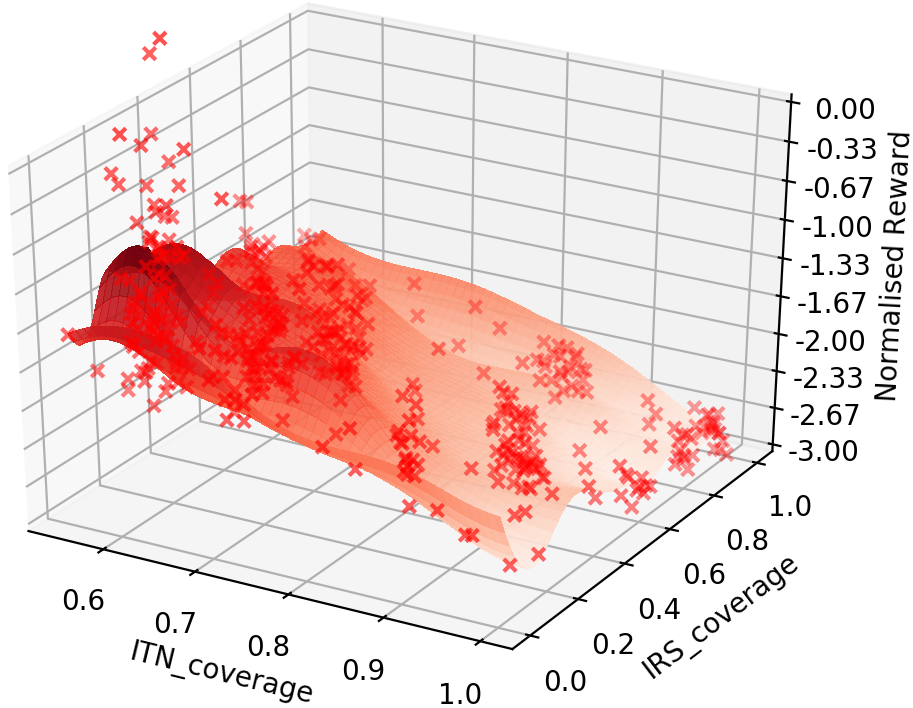
\includegraphics[width=.7\textheight, trim={0 1.8cm 1.5cm 0}, clip=True]{images/Batch_7.png}

\end{frame}



\section{An Example Notebook}



% All of the following is optional and typically not needed. 
\appendix
\section<presentation>*{\appendixname}
\subsection<presentation>*{For Further Reading}

\begin{frame}[allowframebreaks]
        \frametitle{References}
        \bibliographystyle{amsalpha}
        \bibliography{refs/iaai.bib}
\end{frame}

\begin{frame}{Gaussian Processes for Sample-Efficiency and Inference}

\begin{itemize}
\item Similar policies should be highly correlated, despite the stochasticity of simulation outcomes  $\{R_\theta(\bm{a})| \bm{a}\in A \}$
\item Vector policies of actions $\bm{a}$ return stochastic scalar Rewards $R(\bm{a}^{1})...R(\bm{a}^{n})$, with mean $\mu(\bm{a}) = E[R(\bm{a})] $, and covariance $ k(\bm{a},\bm{a}')=E[(R(\bm{a})-\mu(\bm{a}))(R(\bm{a}')-\mu(\bm{a}'))]$
\item A Gaussian Process (GP) can be specified by these mean and covariance functions $GP(\mu(\bm{a}),k(\bm{a},\bm{a}'))$


\end{itemize}

In this case we sample the actions space $A$ and receive corresponding stochastic Rewards $R$ to train a Gaussian Process which can infer with confidence bounds the performance of actions across the Policy space \cite{Williams1996}.  



\end{frame}

\begin{frame}{Gaussian Processes for Sample-Efficiency and Inference}
The learnt parameters describe the posterior distribution over $R(\bm{a})$:

\begin{equation}
\mu_{i+1}(\bm{a}) = \bm{k}_i(\bm{a})^{T}(\bm{K}_{i}+\sigma^2\bm{I})^{-1}R_i
\end{equation}
\begin{equation}
\sigma_{i+1}(\bm{a}) = k(\bm{a},\bm{a}') - \bm{k}_i(\bm{a})^{T}(\bm{K}_{i}+\sigma^2\bm{I})^{-1}\bm{k}_i(\bm{a})
\end{equation}
At each location $\bm{a} \in A$,  $\bm{k}_i(\bm{a})=[k(\bm{a}_i^k,\bm{a})]_{\bm{a}_i^k\in A_i}$ and $\bm{K}_i = [k(\bm{a},\bm{a}')]_{\bm{a},\bm{a}'\in A_i}$, here $\sigma^2$ is the likelihood variance of the GP posterior. For this specific problem we have used a 0-mean function $\mu_0 \equiv 0$ and a Matern-5/2 covariance function or kernel $k(\bm{a},\bm{a}')$, of length scale $=l$ and parameter $\nu = 5/2$.


\end{frame}



%\subsubsection{Upper/Lower Confidence Bound (GP-ULCB)}
\begin{frame}{Upper/Lower Confidence Bound (GP-ULCB)}

\begin{itemize}
\item We introduce the Gaussian Process Upper/Lower Confidence Bound  (GP-ULCB) algorithm, inspired by Gaussian Process Regression (GPR) and work on Upper Confidence Bound (UCB) solutions to the multi-armed bandit problem 
\cite{Auer2010}\cite{Auer2002}. 
\item Combining the natural confidence bounds of Gaussian Processes for stochastic multi-armed bandit problems, and variants have already been proposed in the form of GP-UCB \cite{Srinivas2009} and GP-UCB-PE \cite{Contal2013}. 
\item The choice of using both Upper and Lower confidence bounds was made due to the stochastic nature of policies, minima and maxima would quickly occur in the policy space necessitating a search for both potentially optimal and bad strategies; by including the sampling of minima the agent may thus be allowed to exhibit risk adverse behaviour in its exploration of the policy space. 

\end{itemize}



\end{frame}



%\subsubsection{Genetic Algorithm}
\begin{frame}{Genetic Algorithm}

\begin{itemize}
\item  GA is a biologically inspired, population-based search technique based on the work \cite{Holland1992}.
\item The algorithm is a meta-heuristic inspired by the process of natural selection.
\item We use the reward generated for a policy as the measure of its fitness, and as OpenMalaria provides a stochastic evaluation for each policy, there is noise in the fitness measure.


% not sure this is needed %\textit{In this approach, populations of polices are evaluated in the OpenMalaria simulation environment, and the fitness of these policies assessed.}


The probability of selection of the $j^{th}$ policy in a generation (Batch), $p^j$, is defined by (\ref{weightedroulettewheel}), where $f^j$ is its fitness, the negative of Reward $R(\bm{a}_i)$ normalised between (0,1).
\begin{equation}
p^j = \frac{f^j}{\sum_{k=1}^{B} f^k}
\label{weightedroulettewheel}
\end{equation}


\item Mimicking biological crossover of chromosomes, the two selected policies are mixed, and one of the resulting policies selected at random
\item Finally, a random subset of the components of each derived policy is perturbed by adding noise
\end{itemize}

\end{frame}

%\subsubsection{Batch Policy Gradient}
\begin{frame}{Batch Policy Gradient}
\begin{itemize}
\item Policy gradients \cite{Sutton1999}, chosen as they are able to handle continuous or very large action spaces in the case of this problem and are robust to stochasticity.
\item In this implementation $R_\theta(\bm{a})$ is approximated by a neural network, policies chosen through $\epsilon$-greedy exploration.

During training the agent will choose the policy $\bm{a}^j$ with probability $\epsilon$:
\begin{equation}
\bm{a}^j = \underset{w \sim A_c}{\tt{argmax}}(\bm{w})  
\end{equation}
While a random policy will be sampled with probability $1-\epsilon$.

\end{itemize}
 Similarly to the GP-ULCB algorithm each $\bm{a}^j$ of the Batch is sampled sequentially such that preceding $\bm{a}_{max}$ in the batch are excluded in choosing the next $\bm{a}^j$ comprising the batch policies for evaluation $\bm{a}_i$
\end{frame}



\begin{algorithm}[]
\SetAlgoLined
\KwResult{$\bm{a}_i$: Policy Batch $i$}
 Input: Discrete policy space $\bm{a} \in A_c$\; GP Priors $\mu_0 = 0$, $\sigma_0,l$\; $B= $BatchSize, $f_m= $mixing factor, $f_c= $masking factor\;\
 \For{i = 1,2,...}{
 reset: $\bm{a}_{upper},\bm{a}_{lower}, A_c$\;
 \For{j = 1,2,..,B.}{
 	\eIf{$j<B \times f_m$}{
 	$\bm{a}_i^j = \underset{a \in A_c}{\mbox{argmax}} \ \mu_{i-1}(\bm{a}) + \beta\sigma_{i-1}(\bm{a})$\\
 	mask: $\bm{a}_{upper}$, $|\bm{a^j}-\bm{a}_{upper}| < l \times f_c$\\
 	update: $\bm{a}_{upper} \notin A_c$
 	}
  	{$\bm{a}_i^j = \underset{a \in A}{\tt{argmin}} \ \mu_{i-1}(\bm{a}) - \beta\sigma_{i-1}(\bm{a})$\\
  	mask: $\bm{a}_{lower}$, $|\bm{a^j}-\bm{a}_{lower}| < l \times f_c$\\
 	update: $\bm{a}_{lower} \notin A_c$
  	}
 }
 Return: $R_{\theta}(\bm{a}_i)$\\
 Update Posterior: mean $\mu_{i}(\bm{a})$, variance $\sigma_{i}(\bm{a})$
 }
 %\caption{GP-ULCB}
\end{algorithm}


\end{document}
